\section{The Basics of Software Testing}\label{sect:btesting}
This section introduces some of the basics of software testing. These will assist in understanding the work documented in later sections. The definitions used in this section are taken from the books \textit{Guide to Advanced Software Testing} by Anne Mette Jonassen Hass\cite{Hass} and \textit{Software Testing Techniques} by Boris Beizer\cite{Beizer}.

Testing is an integral part of the software development process at large. It is included in many different software process models. But, what is testing exactly? Hass defines it as follows:
\begin{quotation} \textit{Testing gathers information about the quality of the object under test.}\end{quotation}
Knowing the quality of a piece of software allows an organization to evaluate, whether it is fit for purpose. If not, test results may guide an effort to increase quality.

Before tests can be executed they must be designed. Design can be done from two different points of view: \emph{Functional} and \emph{Structural}. With functional, software is treated like a black box receiving input and computing output. Tests are designed to verify, whether the software conforms to specified behaviour. Structural involves designing test based on the internal structure of the software. Here a tester could for instance test how a piece of code logically branches during execution. The structural approach is often used, when testing individual components. Functional is more apt to use, when testing a set of integrated units or an entire system.

During the software testing process a system is usually tested at different structural levels. During component testing, each component of the system is tested in isolation. This usually requires the implementation of stubs and drivers. A stub simulates the code called by the component, while the driver simulates code, which the component is called by. The size of a component is defined by the organization, in which the code is tested. However, we can usually define a component as an aggregation of units. A Unit is the smallest testable part of a system, and it is itself defined to be a component. The testing of a single unit is often refered to as unit testing. The difference between unit and component testing is that component testing considers not only units but also aggregated components. Through component testing we verify the quality of each component. Once verified we begin to integrate the components with each other. Here integration testing may be performed. This type of test verifies the quality of the communication between the different components. After the system has been fully integrated, testers can perform system testing. At this level of testing, we test the system as a whole. Thorough testing usually involves testing the software at each structual level in the order just described.

As with any other process, testing is restricted by both time and resources available. These greatly affect the quality of testing performed, often called test coverage. Because of this, testers are almost never able to perform exhaustive testing, where all combinations of input and preconditions are tested. Instead, testers select the most important areas to focus on during testing.

Tools are often used to assist in the testing process. An example is the testing framework, which assist in the automatic execution of tests. By the push of a button, a framework can execute a set of user-defined test cases, setting up and tearing down objects as needed. A test case is a well defined set of preconditions and input given to a component. This is accompanied by a set of expected output and postconditions. It passes or fails, depending whether actual output and postconditions match expectations. The required test coverage is often acquired by designing a set of test cases. An advantage of frameworks is that testers can spend more time on test design. Less time will have to be spend on how to implement tests. In theory this leads to testing of a higher quality.

Another bonus of using a framework is that it allows for regression testing. This becomes mostly relevant in the maintenance part of the software life cycle. During this time, new features may be added and bugs fixed. Testers want to ensure that such changes do not lead to regression, where software quality deteriorates. With a framework, regression testing is simple. Once a set of test cases have been set up, they can be run after a change has been made. This will then gauge whether regression has occurred.

\begin{figure}
\centering
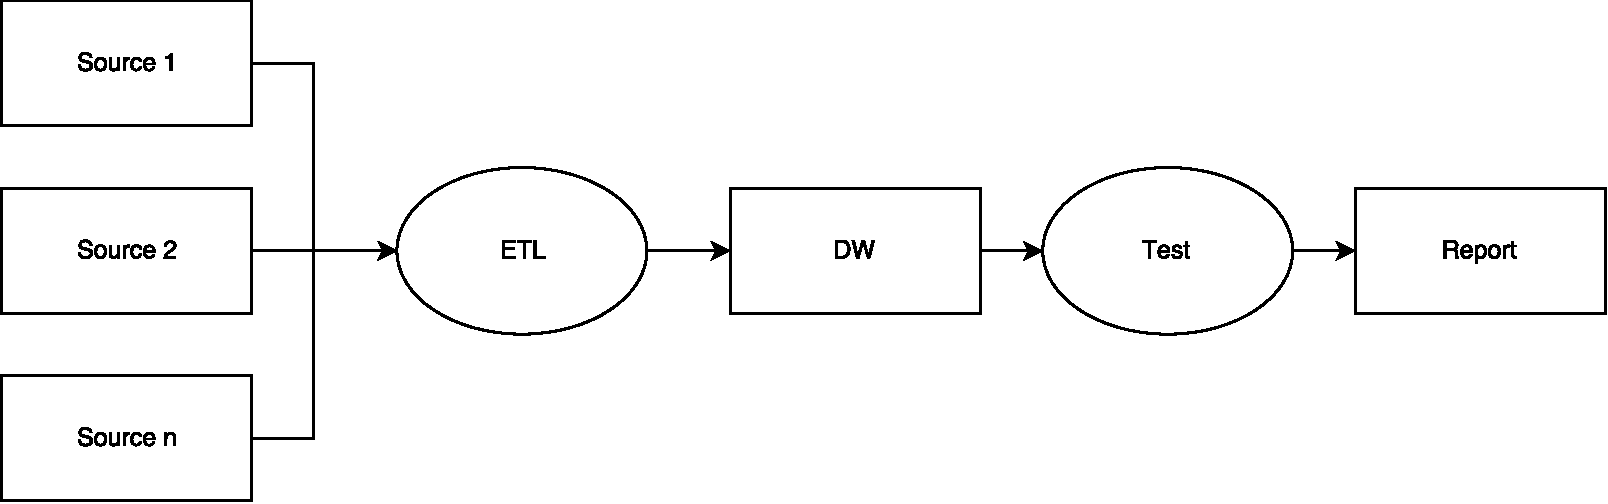
\includegraphics[width=0.5\textwidth]{figures/scenario.pdf}
\caption{Diagram of source to target test}
\label{fig:sourcetotarget}
\end{figure}

A common way to test ETL programs is source to target testing, which validatse whether the data in a populated DW conforms to expectations. It is illustrated in \cref{fig:sourcetotarget}. Here the ETL program under test populates a DW using a set of sources. Once the process has been finished, we test and report on whether assertions about the resulting DW have been met. Assertions concern properties of the DW and its tables such as table length, constraints and so on. This is a system level test, performed once the ETL program has been fully integrated. It is a functional test, as it does not test according to the internal structure of the system. Testing is performed according to system requirements. This method is also ideal for regression testing, as old assertions about DWs can simply be checked again.

